\chapter{使用Git进行版本控制}
\label{cp:git}

\note{本人多年前就接触过Git的使用方法,相关记录可以查看本人的GitHub账号(\href{https://github.com/jstar0}{@jstar0}),并用它进行过\CJKfontspec{STKaiti}代码托管、持续集成(自动化构建和部署)、项目管理、提PR、SaaS对接等操作。\CJKfontspec{SimHei}因此在本报告中,对Git相关操作描述可能相对简略。\CJKfontspec{FangSong}当然,经过系统学习,我对Git的掌握更加熟练和深入了。}

\section{理论基础}

\subsection{Git的基本模型}

Git使用\textbf{对象和引用}的方式来管理版本控制。对象是Git中最基本的单位,包括三种类型:\textbf{blob}、\textbf{tree}和\textbf{commit}。其中,blob是文件内容,tree是目录结构,commit是提交信息。而引用是指向对象的指针,包括分支、标签等。通过对象和引用的方式,实现了Git的基本模型,包含三个基本区域:\textbf{工作区、暂存区和版本库}。工作区是指用户进行编辑的区域,暂存区是指用户准备提交的地方,版本库用于存储历史记录。\\

此部分参考了\citep{MissingSemester}的概念,仅作简述。

\subsection{整理Git的基本操作}

我们将\textit{远程操作}和\textit{本地操作}分开研究,这是基于我们实用性的考量。在远程操作中,我们主要关注\textbf{克隆、推送、拉取}等操作,而在本地操作中,我们主要关注\textbf{初始化库、添加、提交、查看、分支}等操作。我们给出两个表格\autoref{tab:git-remote-operations}和\autoref{tab:git-local-operations}\\

\textbf{远程操作}:\\

\begin{longtable}{c|p{5cm}<{\centering}|p{8cm}<{\centering}}
    \caption{Git远程操作一览表} \label{tab:git-remote-operations} \\
    \toprule
        \textbf{操作名} & \textbf{命令} & \textbf{简介} \\
    \midrule
    \endfirsthead
    \caption[]{Git远程操作一览表(续)} \\
    \toprule
        \textbf{操作名} & \textbf{命令} & \textbf{简介} \\
    \midrule
    \endhead
    \midrule
    \endfoot
    \bottomrule
    \endlastfoot
        克隆 & \verb|git clone <url>| & 从远程仓库克隆到本地 \\
        推送 & \verb|git push| & 将本地提交推送到远程仓库 \\
        拉取 & \verb|git pull| & 从远程仓库拉取最新版本 \\
        获取 & \verb|git fetch| & 从远程仓库获取最新版本 \\
        指定远程 & \verb|git remote| & 查看远程仓库 \\
        分支 & \verb|git branch| & 查看分支 \\
\end{longtable}

\textbf{本地操作}:\\

\begin{longtable}{c|p{5cm}<{\centering}|p{8cm}<{\centering}}
    \caption{Git本地操作一览表} \label{tab:git-local-operations} \\
    \toprule
        \textbf{操作名} & \textbf{命令} & \textbf{简介} \\
    \midrule
    \endfirsthead
    \caption[]{Git本地操作一览表(续)} \\
    \toprule
        \textbf{操作名} & \textbf{命令} & \textbf{简介} \\
    \midrule
    \endhead
    \midrule
    \endfoot
    \bottomrule
    \endlastfoot
        初始化 & \verb|git init| & 初始化一个Git仓库 \\
        添加 & \verb|git add <file>| & 将文件添加到暂存区 \\
        提交 & \verb|git commit -m <message>| & 将暂存区的文件提交到版本库 \\
        查看 & \verb|git status| & 查看当前状态 \\
        分支 & \verb|git branch| & 查看分支 \\
\end{longtable}

\section{实践操作}

\subsection{初始化一个仓库}

要初始化一个仓库,我们可以选择\textit{直接从本地初始化}或者\textit{从远程仓库克隆}。从本地初始化的操作如下:

\begin{listing}[!htpb]
    \begin{minted}{bash}
        git init
    \end{minted}
    \caption{INITialize(初始化)一个Git仓库}
\end{listing}

而若要从云端创建一个仓库并克隆到本地,以GitHub为例,我们先在云端创建一个仓库,如下图:

\begin{figure}[!h]
    \centering
    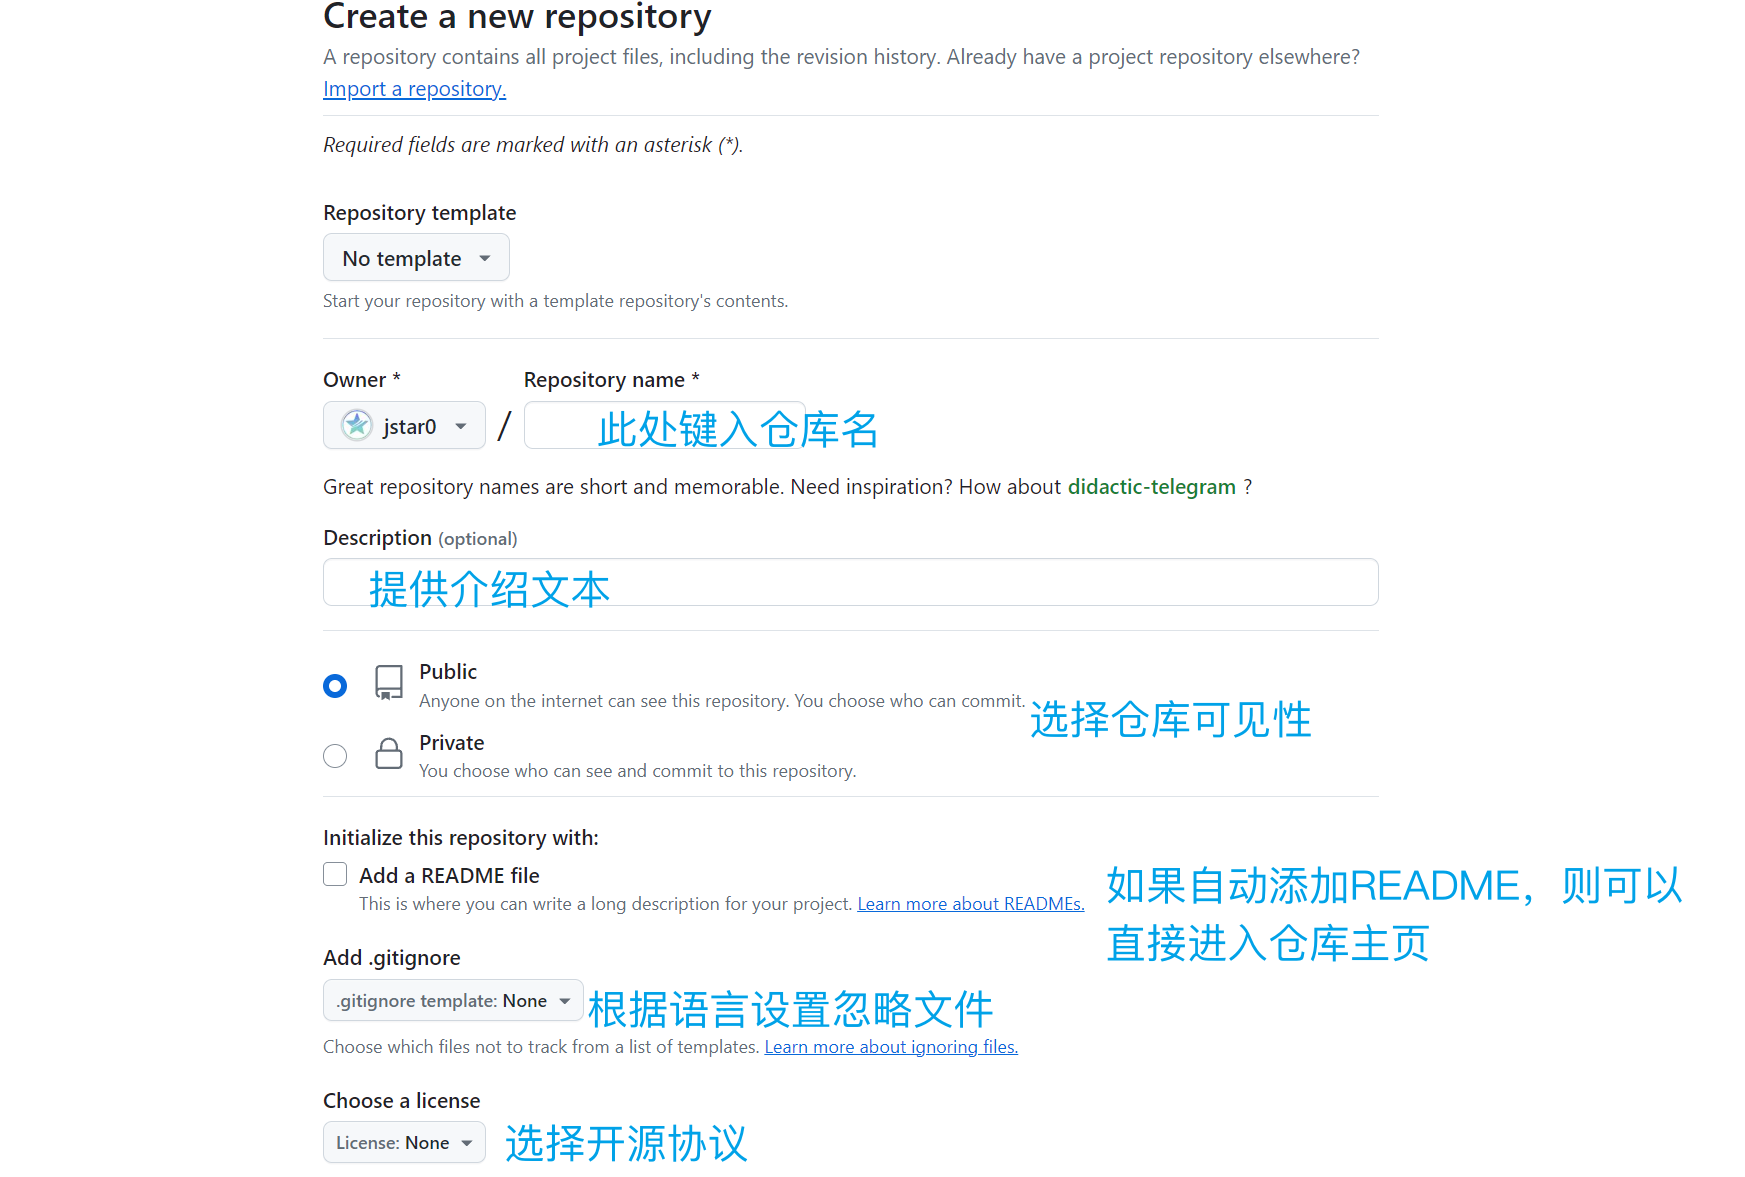
\includegraphics[width=0.65\textwidth]{figures/github-create-repo.png}
    \caption{在GitHub上创建一个仓库}
    \label{fig:github-create-repo}
\end{figure}

然后,我们可以使用\verb|git clone|命令将仓库克隆到本地:

\begin{listing}[!htpb]
    \begin{minted}{bash}
        git clone <url>
    \end{minted}
    \caption{CLONE(克隆)一个Git仓库}
\end{listing}

\subsection{添加、提交和查看}

在仓库中,最基本的操作就是,\textit{添加文件、提交文件,以及查看当前状态}。添加文件会将文件添加到\textbf{暂存区},而提交文件会将暂存区的文件提交到\textbf{版本库}。添加文件的操作如下:

\begin{listing}[!htpb]
    \begin{minted}{bash}
        git add <file>
    \end{minted}
    \caption{ADD(添加)文件到暂存区}
\end{listing}

如需提交所有文件,可以使用\texttt{*}(通配符),或者在不使用此指令而是使用\texttt{git commit -a}命令。但注意,使用此指令或许会造成不希望的结果。提交文件的操作如下:

\begin{listing}[!htpb]
    \begin{minted}{bash}
        git commit -m <message>
    \end{minted}
    \caption{COMMIT(提交)文件到版本库}
\end{listing}

注意,上述指令中\texttt{-m}参数可以留空,不过后期会自动打开一个文件要求输入Commit信息。查看当前状态的操作如下:

\begin{listing}[!htpb]
    \begin{minted}{bash}
        git status
    \end{minted}
    \caption{STATUS(状态)查看当前状态}
\end{listing}

上述操作是Git中最基本的操作,我们在本地创建一个仓库作为示例,如下图:

\begin{figure}[!h]
    \centering
    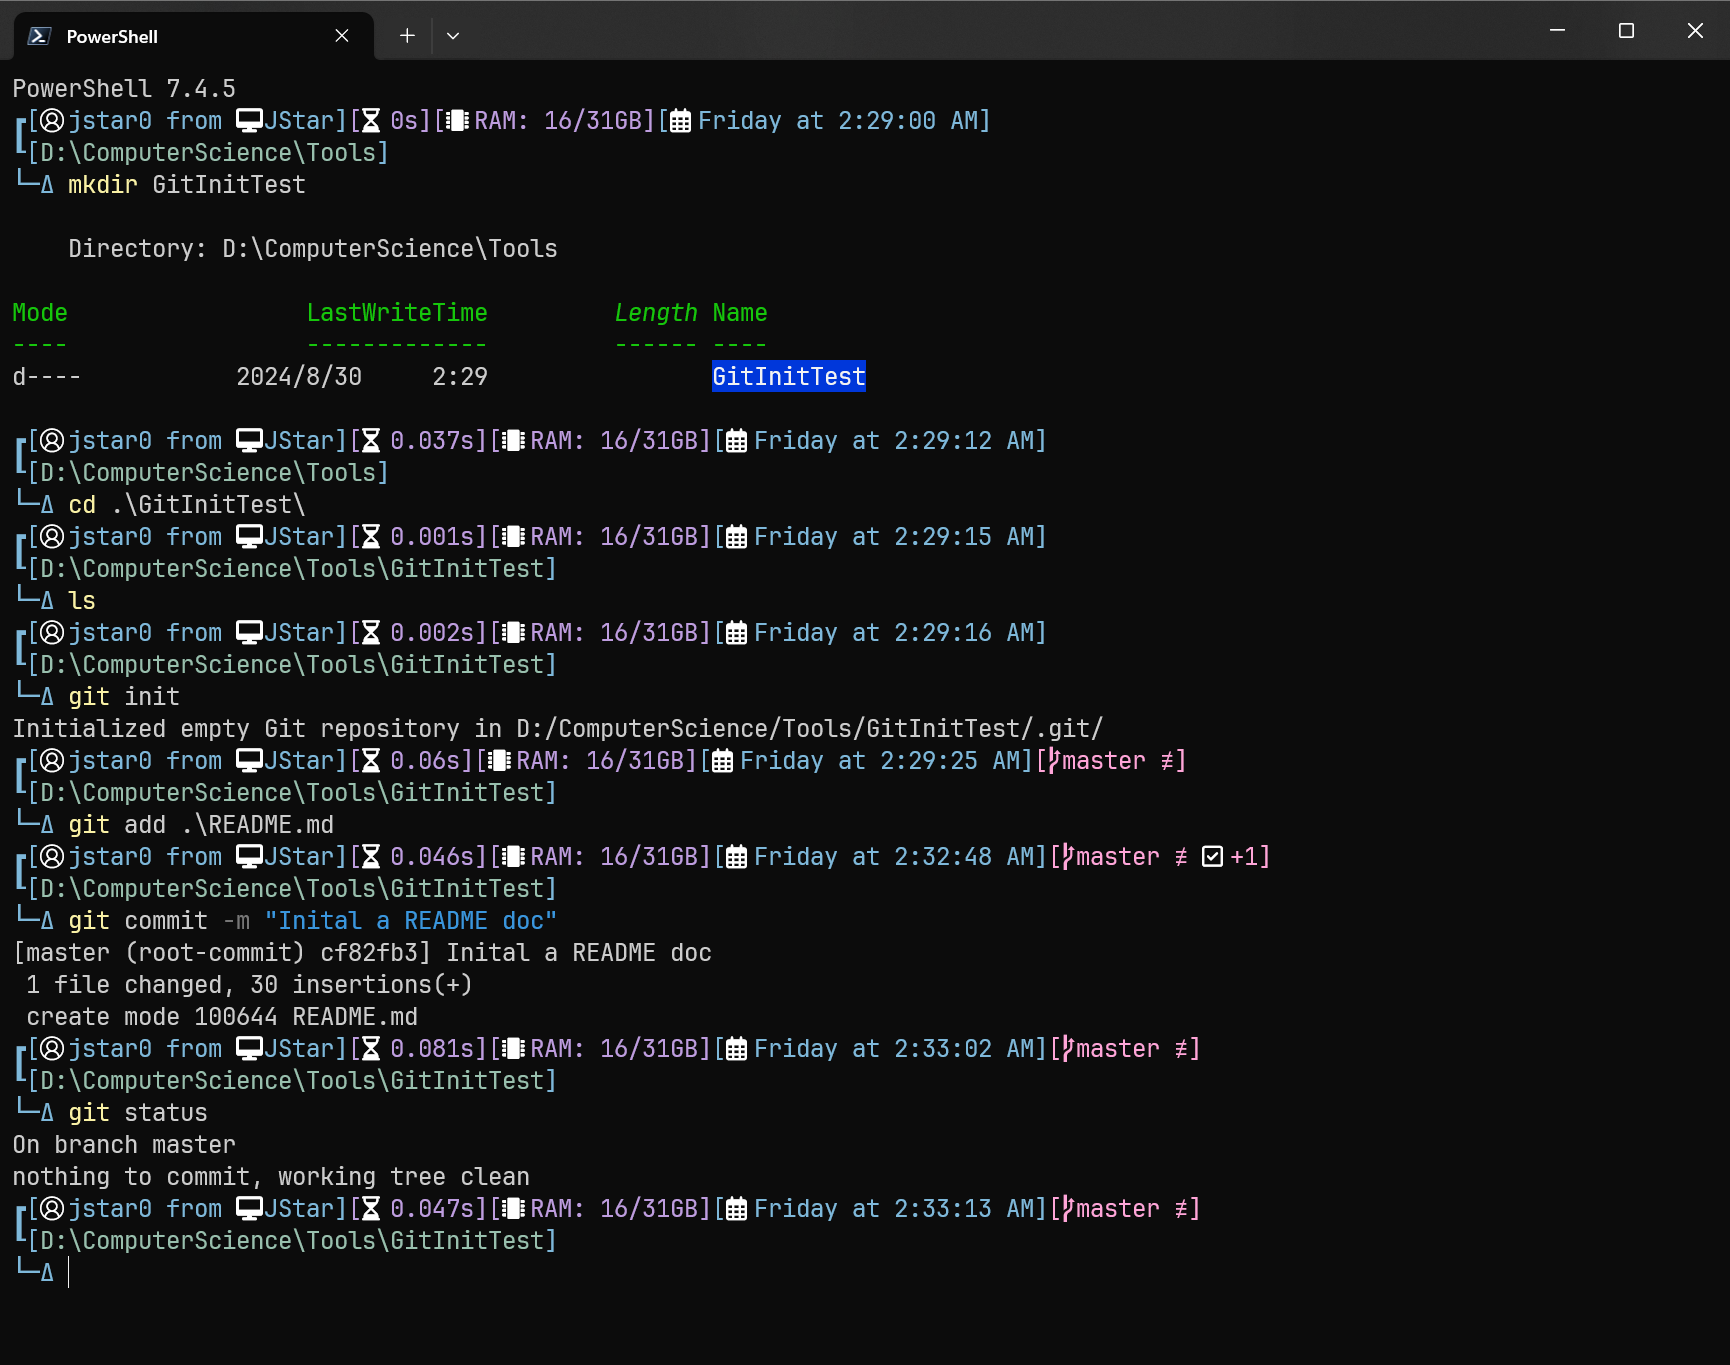
\includegraphics[width=0.65\textwidth]{figures/git-local-operations.png}
    \caption{本地操作创建、提交示例}
    \label{fig:git-local-operations}
\end{figure}

如果要查看提交的历史记录,可以使用\texttt{git log}命令。此命令会列出所有的提交记录,包括提交者、提交时间、提交信息等。如果要查看某个文件的提交历史,可以使用\texttt{git log <file>}命令。

一般的,我们都会使用\texttt{.gitignore}文件来忽略一些不必要的文件,如\texttt{.DS\_Store}、\texttt{.vscode}等。我们可以在\texttt{.gitignore}文件中添加这些文件,比如我们:

\begin{listing}[h!]
    \begin{minted}{bash}
        echo ".vscode/" >> .gitignore
    \end{minted}
    \caption{添加.vscode文件夹到.gitignore}
\end{listing}

就可以忽略\texttt{.vscode}文件夹了。此处\textit{忽略}的意思是,Git不会将这些文件夹或文件添加到版本库中。具体的正则、匹配写法,可以参考\href{https://git-scm.com/docs/gitignore}{Git官方文档}。

\subsection{推送到远端、拉取最新版本}

在本地操作完成后,我们可以将本地的提交推送到远程仓库,或者从远程仓库拉取最新版本。\\

通常,我们直接编辑从云端clone下来的仓库,在这种情况下的拉取和推送操作如下:

\begin{listing}[!htpb]
    \begin{minted}{bash}
        git pull # 拉取最新版本
        git push # 推送到远程仓库
    \end{minted}
    \caption{PULL(拉取)和PUSH(推送)操作}
\end{listing}

然而,如要将本地的仓库推送到远程仓库,我们需要先指定远程仓库,然后再推送。指定远程仓库的操作如下:

\begin{listing}[!htpb]
    \begin{minted}{bash}
        git remote add origin <url>
        git remote -v # 验证远程仓库
    \end{minted}
    \caption{REMOTE(远程)添加远程仓库}
\end{listing}

然后,我们可以推送到远程仓库:

\begin{listing}[!htpb]
    \begin{minted}{bash}
        git push -u origin master # 关联远程仓库分支并推送
    \end{minted}
    \caption{PUSH(推送)到远程仓库}
\end{listing}

其中,\texttt{-u}参数表示\textit{upstream},即将本地的\texttt{master}分支与远程的\texttt{master}分支关联起来。这样,我们在后续的推送和拉取操作中,就可以省略\texttt{origin master}参数了。\\

特别的,我遇到的问题是,如果本地未配置SSH密钥,那么在推送时会出现\texttt{Permission denied}的错误。这时,我们需要配置SSH密钥,参考\href{https://docs.github.com/en/github/authenticating-to-github/connecting-to-github-with-ssh}{GitHub官方文档}。\\

使用Git Bash进行如下操作:

\begin{listing}[!h]
    \begin{minted}{bash}
        ssh-keygen -t rsa -b 4096 -C "MyEmail@example.com" # 生成SSH密钥
        eval $(ssh-agent -s) # 启动ssh-agent
        ssh-add ~/.ssh/id_rsa # 添加SSH密钥
        # 然后将SSH密钥添加到GitHub账号中
        cd ~/.ssh
        cat id_rsa.pub # 查看公钥
    \end{minted}
    \caption{配置SSH密钥}
\end{listing}

此时再行推送,一切正常。

\subsection{分支操作}

分支是一个相当重要的概念。我们可以通过分支来实现\textit{并行开发},在不同的分支上进行不同的开发,然后再合并到主分支上。\\

首先我们提供分支相关的基本操作。

\begin{listing}[!htpb]
    \begin{minted}{bash}
        git branch # 查看目前的所有分支
        git branch <branch-name> # 创建一个分支
        git checkout <branch-name> # 切换到一个分支
        git merge <branch-name> # 从<branch-name>合并到当前分支
        git branch -d <branch-name> # 删除<branch-name>分支
    \end{minted}
    \caption{BRANCH(分支)操作}
\end{listing}

而在实际操作中,如果要快速创建并切换分支,可以使用如下命令:

\begin{listing}[!htpb]
    \begin{minted}{bash}
        git checkout -b <branch-name> # 创建并切换分支
    \end{minted}
    \caption{BRANCH(分支)创建并切换分支}
\end{listing}

一般的,我们会在\texttt{master}分支上创建一个新的分支,然后在新的分支上进行开发。开发完成后,我们可以将新的分支合并到\texttt{master}分支上。\\

如果遇到冲突,我们需要手动解决冲突。此时,Git会在冲突的文件中标记出冲突的地方,我们需要手动解决这些冲突。解决冲突后,我们需要将文件标记为\textit{已解决},然后再提交。\\

而如果我此刻在处理一些文件,突然遇到紧急的问题,需要切换到\texttt{master}分支,可以使用\texttt{git stash}命令,将当前的工作区保存到\texttt{stash}中,然后切换到\texttt{master}分支。在处理完紧急问题后,我们可以使用\texttt{git stash pop}命令,将\texttt{stash}中的工作区恢复。这个过程称作\textbf{贮藏}\\

如果要\textbf{清理}掉所有未被跟踪的文件,可以使用\texttt{git clean -f}命令,以清理掉所有未被跟踪的文件,包括\texttt{.gitignore}中忽略的文件。如果要清理掉所有未被跟踪的文件和文件夹,可以使用\texttt{git clean -fd}命令。具体参见\citep{Stash&Clean}。\\

下面给出一个分支操作的实例:(见\autoref{listing:git-branch-example})

\begin{longlisting}
    \begin{minted}{bash}
        # 目前在master分支上
        git branch
        # * main
        git branch hotfix
        git checkout hotfix
        # Switched to branch 'hotfix'
        # 或者直接使用 git checkout -b hotfix
        git status
        # On branch hotfix
        # nothing to commit, working tree clean
        # 我们发现此时已经在hotfix分支上了,对hotfix分支进行一些修改
        echo "some changes" > hotfix.txt
        git add .\hotfix.txt
        git commit -m "Add hotfix.txt"
        # [hotfix 82b935a] Add hotfix.txt
        # 1 file changed, 1 insertion(+)
        # create mode 100644 hotfix.txt
        git checkout main
        # Switched to branch 'main'
        git merge hotfix
        # Updating 57433c9..82b935a
        # Fast-forward
        # hotfix.txt | 1 +
        # 1 file changed, 1 insertion(+)
        # create mode 100644 hotfix.txt
        # 我们发现,hotfix分支已经合并到main分支上了
        # 这只是最简单的情况,两个分支并没有文件冲突(即hotfix分支中的文件和main分支中的文件在分支后没有同时被修改)
    \end{minted}
    \caption{Git分支操作示例其一}
    \label{listing:git-branch-example-1}
\end{longlisting}

进行\texttt{merge}操作前后的区别如下图:

\begin{figure}[!h]
    \centering
    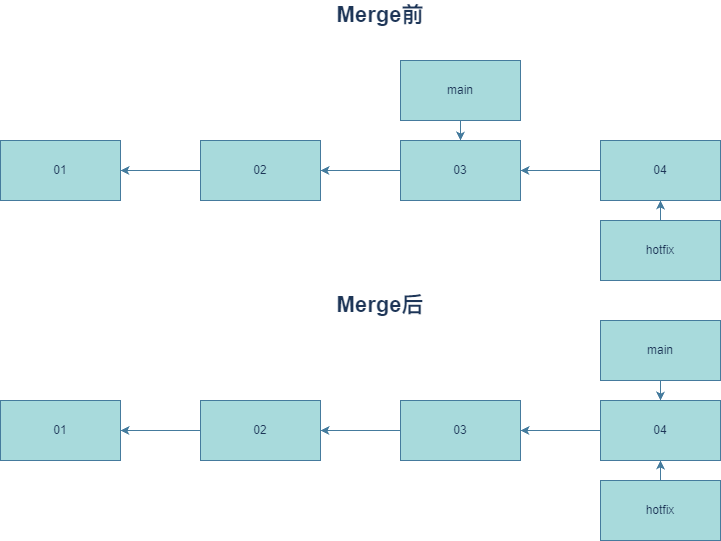
\includegraphics[width=0.65\textwidth]{figures/git-branch-1.png}
    \caption{分支合并前后的区别}
    \label{fig:git-branch-merge}
\end{figure}

现实情况往往更加复杂,如果在分支出现后,两者同时修改了同一个文件,就会出现冲突。此时,我们需要手动解决冲突,然后再提交。解决冲突可以是手动修改文件,也可以使用\texttt{git mergetool}命令等,具体参见\citep{MergeConflict}。

\section{总结与感悟}

Git是非常强大的版本控制工具,在实际开发中,我们通过使用Git来进行版本控制,实现\textit{并行开发}、\textit{版本回退}、\textit{代码合并}等操作。实际上,VS Code也提供了强大的Git支持,在使用VS Code进行代码编辑时,也可以体会这种带GUI界面的便捷性。\\

通过本次实践,我对Git的操作有了更深入的了解,包括\textit{初始化仓库}、\textit{添加、提交、查看}、\textit{推送、拉取}、\textit{分支操作}等。\textit{工欲善其事,必先利其器。}如果能熟练运用Git,我们就能够更好地维护代码,提高开发效率,减免错误发生。